\documentclass[UTF8,a4paper,11pt]{ctexart}

\usepackage[left=2.25cm,right=2.25cm,top=2.15cm,bottom=2.35cm]{geometry}
\usepackage{amsmath,amssymb}
\usepackage{graphicx}
\usepackage{booktabs}
\usepackage{tabularx}
\usepackage{array}
\usepackage{xcolor}
\usepackage{hyperref}
\usepackage{xurl}
\usepackage{enumitem}
\usepackage{caption}
\usepackage{subcaption}
\usepackage{listings}
\usepackage{fancyhdr}
\usepackage{lastpage}
\usepackage{titlesec}
\usepackage{tocloft}
\usepackage{setspace}
\usepackage{float}
\usepackage{tikz}
\usetikzlibrary{arrows.meta,positioning,shapes.geometric}
\usepackage{makecell}
\usepackage{indentfirst}

\hypersetup{colorlinks=true,linkcolor=black,urlcolor=blue,citecolor=black}
\urlstyle{same}
\linespread{1.20}
\setlength{\parindent}{2em}
\setlength{\parskip}{0.10em}
\setlength{\emergencystretch}{3em}
\setlist[itemize]{leftmargin=2.0em,itemsep=0.03em,topsep=0.12em}
\captionsetup{font=small,labelfont=bf,labelsep=space}
\renewcommand{\arraystretch}{1.12}
\newcolumntype{Y}{>{\raggedright\arraybackslash}X}
\newcolumntype{L}[1]{>{\raggedright\arraybackslash}p{#1}}
\newcolumntype{C}[1]{>{\centering\arraybackslash}p{#1}}
\newcommand{\file}[1]{\texttt{#1}}

\definecolor{codebg}{HTML}{F7F7F7}
\lstset{basicstyle=\ttfamily\small,breaklines=true,frame=single,backgroundcolor=\color{codebg},columns=fullflexible,showstringspaces=false,keepspaces=true,aboveskip=0.45em,belowskip=0.45em}

\pagestyle{fancy}
\fancyhf{}
\fancyhead[L]{\small 人工智能导论 - 可解释的谣言检测大作业报告}
\fancyhead[R]{\small 第 6 组}
\fancyfoot[C]{\small 第 \thepage 页 / 共 \pageref{LastPage} 页}
\renewcommand{\headrulewidth}{0.4pt}
\setlength{\headheight}{15pt}

\titleformat{\section}{\centering\heiti\zihao{3}}{\thesection}{0.8em}{}
\titleformat{\subsection}{\heiti\zihao{4}}{\thesubsection}{0.7em}{}
\titlespacing*{\section}{0pt}{0.75em}{0.55em}
\titlespacing*{\subsection}{0pt}{0.55em}{0.25em}
\renewcommand{\contentsname}{目录}
\renewcommand{\cftsecleader}{\cftdotfill{\cftdotsep}}
\renewcommand{\cftsubsecleader}{\cftdotfill{\cftdotsep}}
\setlength{\cftbeforesecskip}{0.22em}
\renewcommand{\cftsecfont}{\heiti}
\renewcommand{\cftsecpagefont}{\heiti}

\begin{document}

\thispagestyle{fancy}
\begin{center}
  \vspace*{0.8cm}
  {\heiti\zihao{2} 上海交通大学《人工智能导论》课程大作业}\\[0.9em]
  {\heiti\zihao{1} 可解释的谣言检测}\\[0.4em]
  {\bfseries\Large Explainable Rumor Detection}\\[2.0em]
\end{center}

\begin{center}
\begin{tabularx}{0.90\textwidth}{>{\heiti}L{2.15cm}Y>{\heiti}L{2.15cm}Y}
完成组号 & 第 6 组 & 完成时间 & 2 周 \\[0.75em]
小组人员 & \makecell[l]{钟国鹏（523150910082）\\曾子恒（523010910022）\\董治衡（524031910250）} & 贡献比例 & \makecell[l]{三人贡献均等\\各约 33.3\%} \\[0.75em]
组长姓名 & 钟国鹏 & 组长学号 & 523150910082 \\[0.75em]
邮箱 & \footnotesize\texttt{i\_promise23@sjtu.edu.cn} & GitHub & \footnotesize\url{https://github.com/ipromise77/explainable-rumor-detection-2026} \\[0.75em]
运行环境 & Python 3.11, scikit-learn & 提交内容 & README, report.pdf, code \\
\end{tabularx}
\end{center}

\vspace{1.0em}
\begin{center}
\begin{tabularx}{0.86\textwidth}{>{\heiti}L{2.5cm}Y}
项目目标 & 输入英文推文，输出二分类标签，其中 0 表示非谣言、1 表示谣言，并给出中文判断依据。 \\[0.5em]
主模型 & 三路 TF-IDF 特征 + Logistic Regression 概率集成，默认不依赖学校 API 或本地缓存。 \\[0.5em]
增强模块 & 备选增强检测器仅在低置信非谣言样本上追加分级话术信号，作为可复现实验补充。 \\
\end{tabularx}
\end{center}

\vfill
\begin{center}
{\small 本组成员贡献均等；远程仓库提交分支为 \texttt{origin/codex/final-submission-polish}。}
\end{center}

\newpage
\tableofcontents
\newpage

\section{任务目标}
本项目完成“可解释的谣言检测”任务：对输入推文输出 $0/1$ 标签、谣言概率和中文判断依据，并保证默认主模型可离线复现。整体流程如下：先统一预处理文本，再完成数据审计、模型训练、解释生成和前端展示；学校 API 与缓存结果只作为探索或增强记录，不作为默认提交依赖。

\begin{center}
\vspace{0.2em}
{\heiti 任务目标流程图}\par\vspace{0.35em}
\begin{tikzpicture}[
  node distance=0.55cm and 0.43cm,
  box/.style={draw=black!65, rounded corners=2mm, align=center, minimum height=0.78cm, inner xsep=4.5pt, inner ysep=4pt, fill=black!2, font=\small},
  goal/.style={draw=black!75, rounded corners=2mm, align=center, minimum height=0.82cm, inner xsep=5pt, inner ysep=4pt, fill=blue!5, font=\small\bfseries},
  arr/.style={-{Latex[length=2.1mm]}, thick, draw=black!65}
]
\node[box] (input) {输入推文\\\texttt{text}};
\node[box, right=of input] (audit) {数据审计\\清洗冲突};
\node[goal, right=of audit] (model) {主模型分类\\标签 + 概率};
\node[box, right=of model] (exp) {局部证据\\中文解释};
\node[box, right=of exp] (demo) {前端演示\\复现提交};
\draw[arr] (input) -- (audit);
\draw[arr] (audit) -- (model);
\draw[arr] (model) -- (exp);
\draw[arr] (exp) -- (demo);
\end{tikzpicture}
\end{center}

\section{具体内容}
\subsection{实施方案}
系统实施分为四步：数据审计、默认主模型训练、解释生成、前端展示。数据审计使用与模型一致的 \texttt{preprocess\_text()} 规则，先把 URL、用户名和 hashtag 等社交媒体元素统一到稳定形式，再检查是否存在“同一输入、相反标签”的冲突；默认主模型 \texttt{RumourDetectClass} 采用三路 TF-IDF 与 Logistic Regression 集成，在普通 CPU 环境下即可训练和预测；解释模块依据局部特征贡献生成中文判断依据；演示页面由 \texttt{scripts/run\_demo\_server.py} 启动，展示标签、概率、来源和解释。整个方案优先保证默认结果离线可复现，增强模型和 LLM 相关结果只作为补充分析，不混入默认主线。

小组分工如下：钟国鹏负责项目和仓库管理、模型构建与修改、report 撰写和后续修改；曾子恒、董治衡负责模型修改完善和 report 修改。三位成员贡献均等。具体协作过程中，组长统一维护远程分支、整理实验结果和最终提交文件；两位组员主要围绕模型效果、解释输出和报告表达提出修改意见，并参与报告多轮检查。这样的分工使代码、结果和论文表述能够保持一致。

数据方面，原始训练集 2840 条，验证集 401 条。预处理包括 HTML 反转义、小写化、URL 归一化为 \texttt{URLTOKEN}、用户归一化为 \texttt{USERTOKEN}、hashtag 展开。如图\ref{fig:data-audit}，审计发现训练集中有 3 组、7 行“归一化后文本相同但标签冲突”的样本，验证集无同类冲突。我们保留原始 \texttt{train.csv}，只额外生成 \texttt{train\_clean.csv}，不修改 \texttt{val.csv}，避免人为提高验证结果。该处理方式的目的不是追求更高分数，而是让训练数据的监督信号更自洽：如果两条文本在模型视角下完全相同，却分别标为 0 和 1，模型无法通过文本特征学习到稳定规律，解释时也难以给出可信依据。

\begin{figure}[htbp]
\centering
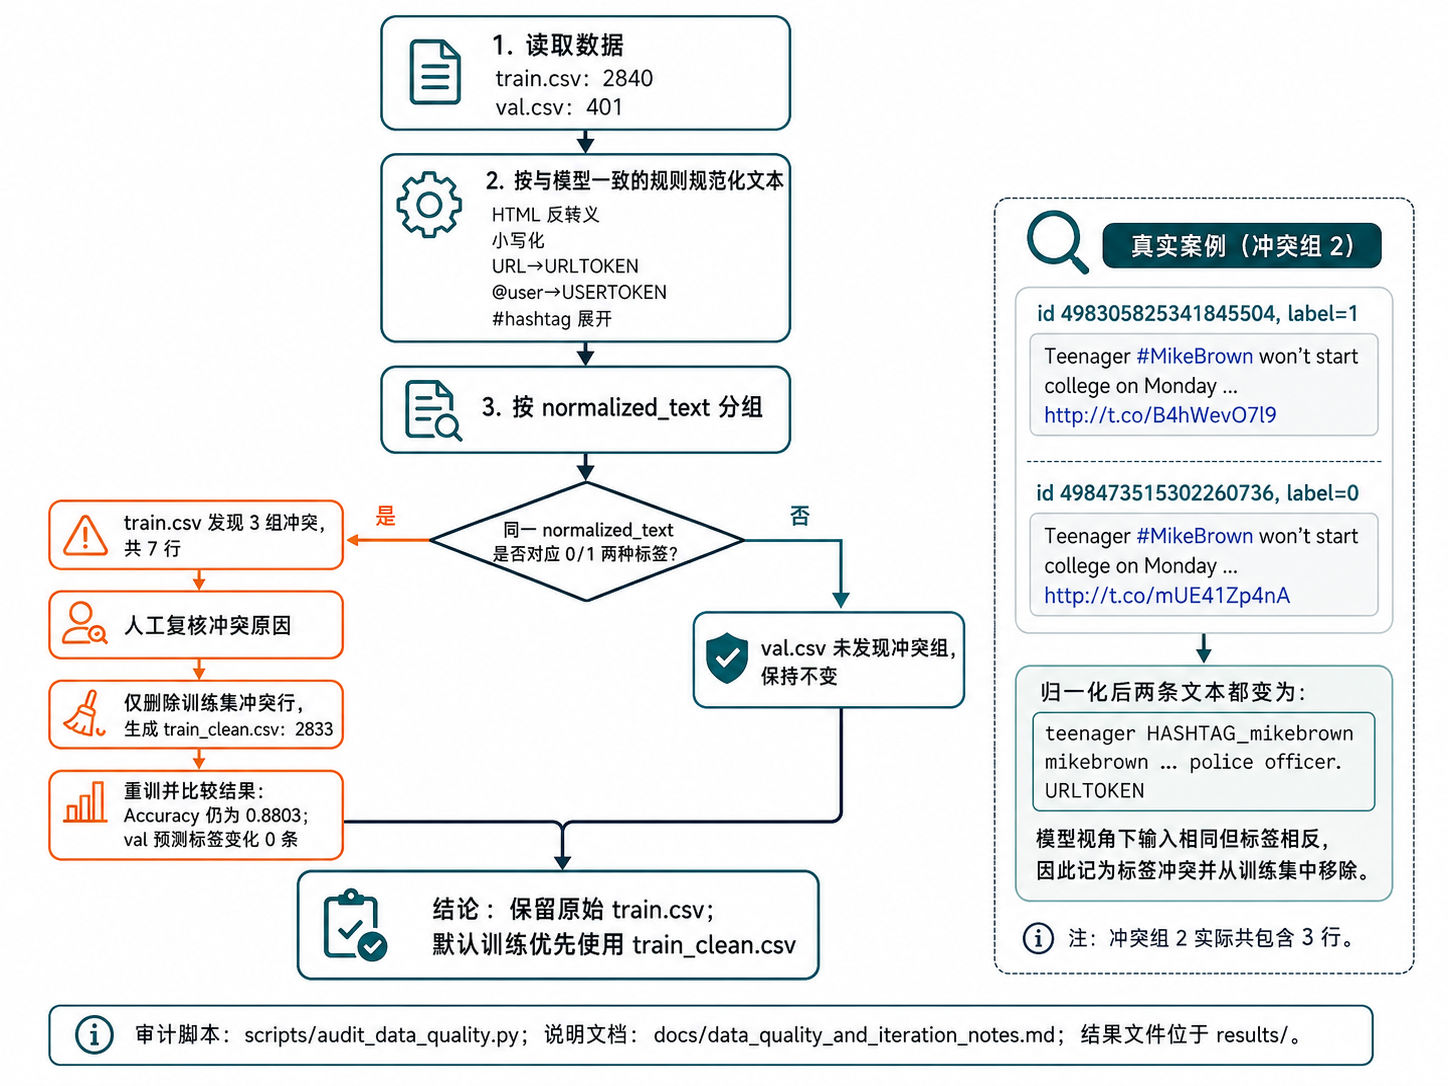
\includegraphics[width=0.90\textwidth]{figures/data_audit_case.png}
\caption{数据集清洗与数据质量审计流程。右侧给出冲突组 2 的真实样本：两条推文仅短链接不同，但归一化后成为同一模型输入，标签却分别为 1 和 0。}
\label{fig:data-audit}
\end{figure}

\subsection{核心代码分析}
核心目录包括 \file{rumer2026/}、\file{src/}、\file{scripts/}、\file{models/}、\file{results/}、\file{demo/} 和 \file{docs/}。\file{rumor\_detector.py} 是默认主模型接口，负责预处理、训练、预测和解释；\file{final\_detector.py} 是备选增强检测器；\file{run\_demo\_server.py} 用于启动本地可视化页面。推荐环境为 Python 3.11，默认主模型不需要 PyTorch。

从代码逻辑看，\file{preprocess\_text()} 是训练、评估、预测和审计共同使用的入口，因此可以避免“训练时一种预处理、预测时另一种预处理”的问题。\file{train\_ensemble()} 按配置训练三个子模型，\file{predict\_proba()} 对三路概率取平均，\file{evidence\_for\_text()} 从稀疏 TF-IDF 向量和逻辑回归权重中提取证据。增强检测器不重写基座模型，而是在本地预测为非谣言且谣言概率较低时才检查分级话术信号，因此可以通过参数关闭，便于教师单独复现默认主模型。

\begin{figure}[htbp]
\centering
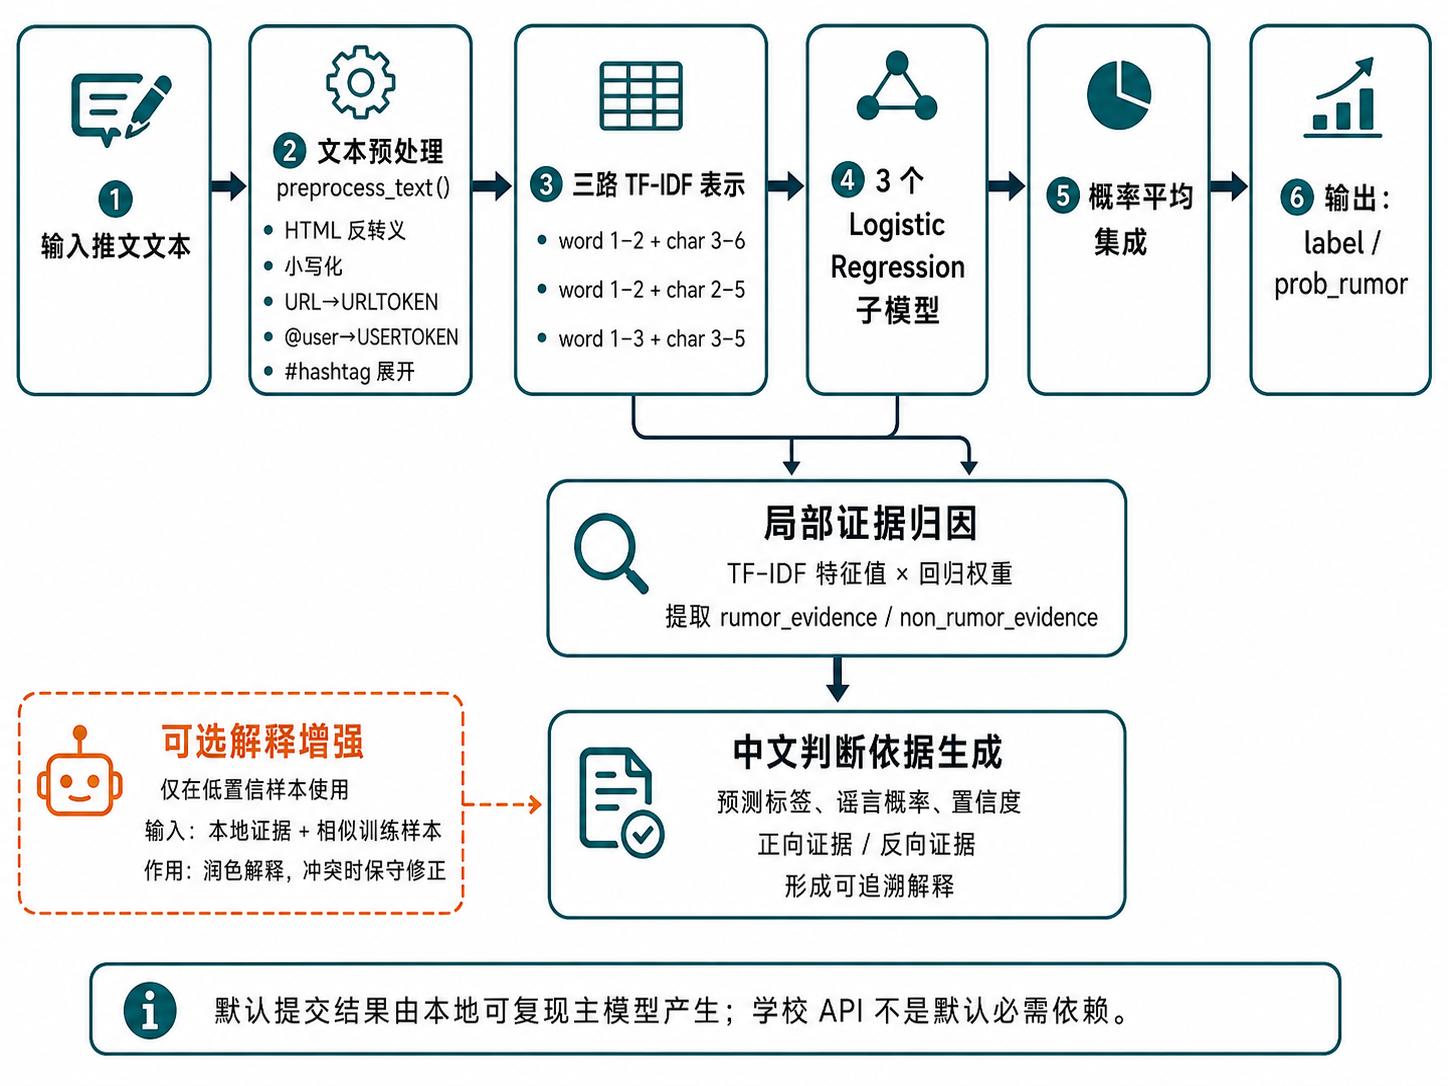
\includegraphics[width=0.93\textwidth]{figures/main_pipeline.png}
\caption{默认主模型与解释增强流程。主线为三路 TF-IDF 表示、三个 Logistic Regression 子模型和概率平均；解释分支使用特征贡献生成中文依据。}
\label{fig:pipeline}
\end{figure}

设输入文本为 $x$，预处理后为 $\tilde{x}=g(x)$。第 $m$ 个子模型构造词级与字符级 TF-IDF 表示
\begin{equation}
\phi_m(\tilde{x})=[\phi_m^{word}(\tilde{x});\phi_m^{char}(\tilde{x})].
\end{equation}
代码采用 sublinear TF 与平滑 IDF：
\begin{equation}
\mathrm{tf}'(t,d)=1+\log \mathrm{tf}(t,d),\quad
\mathrm{idf}(t)=\log\frac{1+n}{1+\mathrm{df}(t)}+1.
\end{equation}
每个子模型为逻辑回归：
\begin{equation}
p_m=P_m(y=1|x)=\sigma(\mathbf{w}_m^\top\phi_m(\tilde{x})+b_m),\quad
\sigma(s)=\frac{1}{1+e^{-s}}.
\end{equation}
最终概率取三路平均，并以 0.5 为阈值：
\begin{equation}
P(y=1|x)=\frac{1}{3}\sum_{m=1}^{3}p_m,\quad
\hat{y}=\mathbb{I}[P(y=1|x)\ge0.5].
\end{equation}
局部解释使用 $c_i=w_i\phi_i(\tilde{x})$，正贡献为支持谣言证据，负贡献为支持非谣言证据。系统不会声称判断新闻事实真假，而是说明模型为什么把文本判到某一类：例如某些词项、字符片段或话题标签贡献更偏向谣言方向，另一些证据则偏向非谣言方向。备选增强器见图\ref{fig:final-detector}，只在窄候选集上检查话术信号，避免大范围规则覆盖。

\begin{figure}[htbp]
\centering
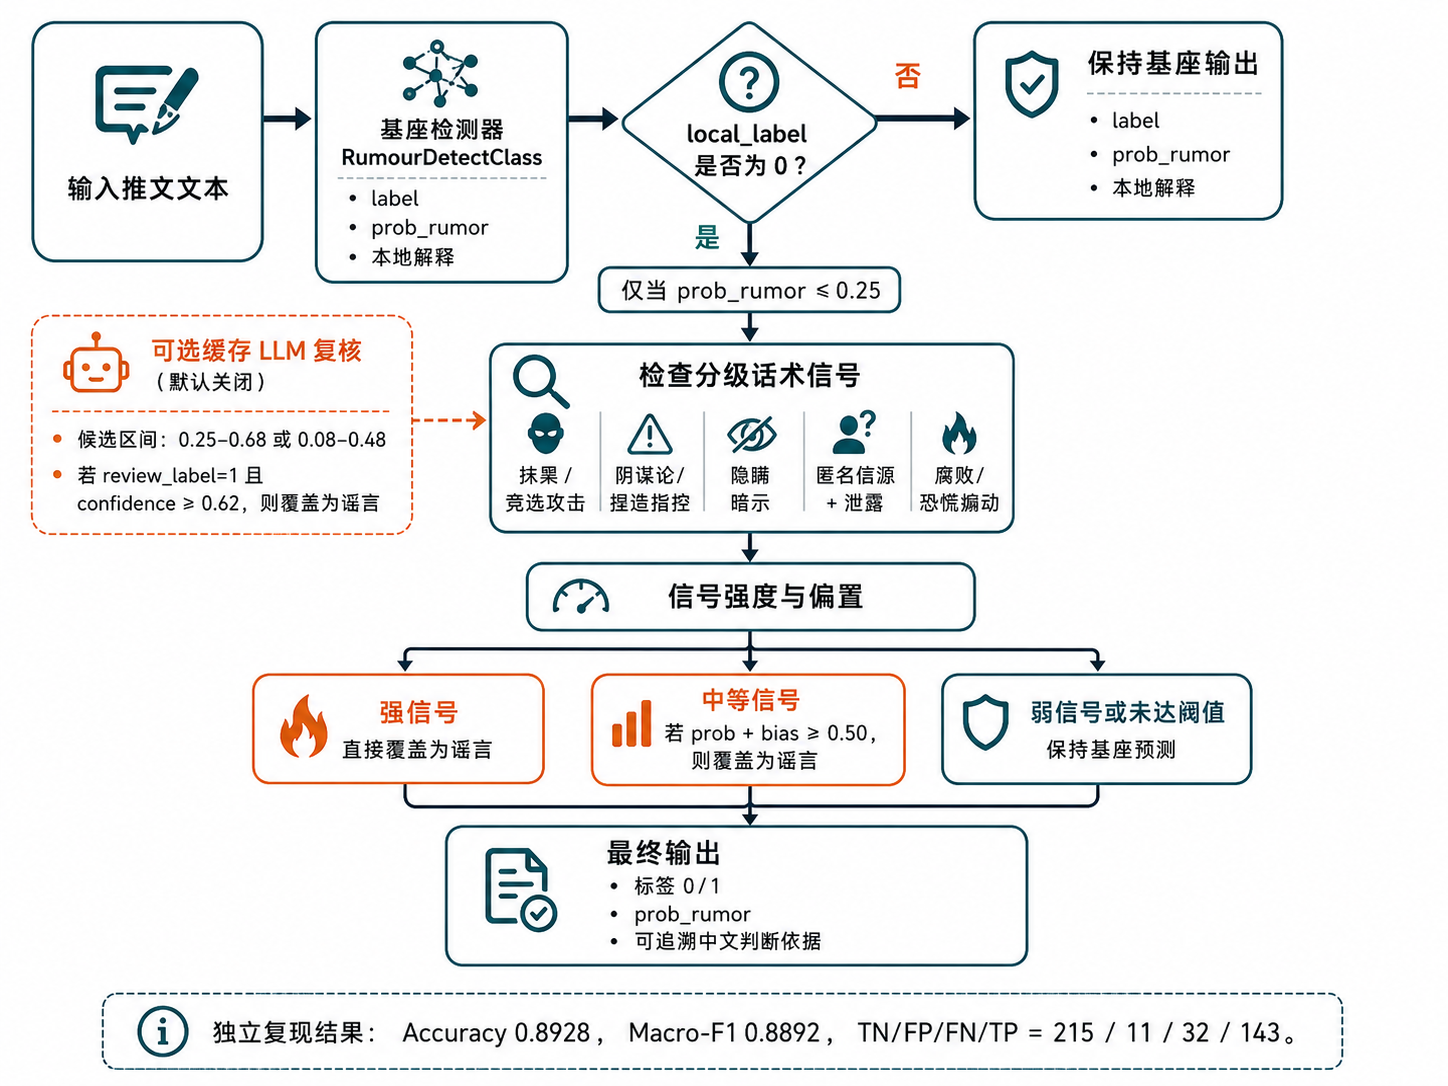
\includegraphics[width=0.90\textwidth]{figures/final_detector_architecture.png}
\caption{备选增强检测器 \texttt{FinalRumourDetectClass}。强信号直接覆盖为谣言，中等信号需满足概率偏置阈值，弱信号保持基座预测。}
\label{fig:final-detector}
\end{figure}

\subsection{检测结果分析与判断依据分析}
默认主模型在 \texttt{val.csv} 上达到 Accuracy 0.8803、Macro-F1 0.8757、Rumor F1 0.8519。备选增强模型默认不读 LLM 缓存，达到 Accuracy 0.8928、Macro-F1 0.8892、Rumor F1 0.8693，混淆矩阵由 [[215, 11], [37, 138]] 改为 [[215, 11], [32, 143]]，说明主要改进来自减少 false negative。我们没有把历史探索中更高但依赖缓存或验证集后处理的结果写成默认指标，因为这会削弱可复现性和评估公平性。报告中所有正式数字均来自仓库结果文件或脚本可重新生成的输出。

\begin{table}[H]
\centering
\caption{验证集结果汇总，混淆矩阵格式为 [[TN, FP], [FN, TP]]}
\begin{tabularx}{\textwidth}{L{2.55cm}C{1.55cm}C{1.55cm}C{1.55cm}Y}
\toprule
方案 & Accuracy & Macro-F1 & Rumor F1 & 说明 \\
\midrule
\makecell[l]{Rumour\\DetectClass} & 0.8803 & 0.8757 & 0.8519 & 默认主模型；[[215, 11], [37, 138]]。 \\
低置信 FN 复核 & 0.8828 & 0.8784 & 0.8554 & 复核候选 79 条，覆盖 1 条，无新增 FP。 \\
\makecell[l]{FinalRumour\\DetectClass} & 0.8928 & 0.8892 & 0.8693 & 默认不读 LLM 缓存；[[215, 11], [32, 143]]。 \\
\bottomrule
\end{tabularx}
\end{table}

\begin{figure}[htbp]
\centering
\begin{subfigure}{0.49\textwidth}
\centering
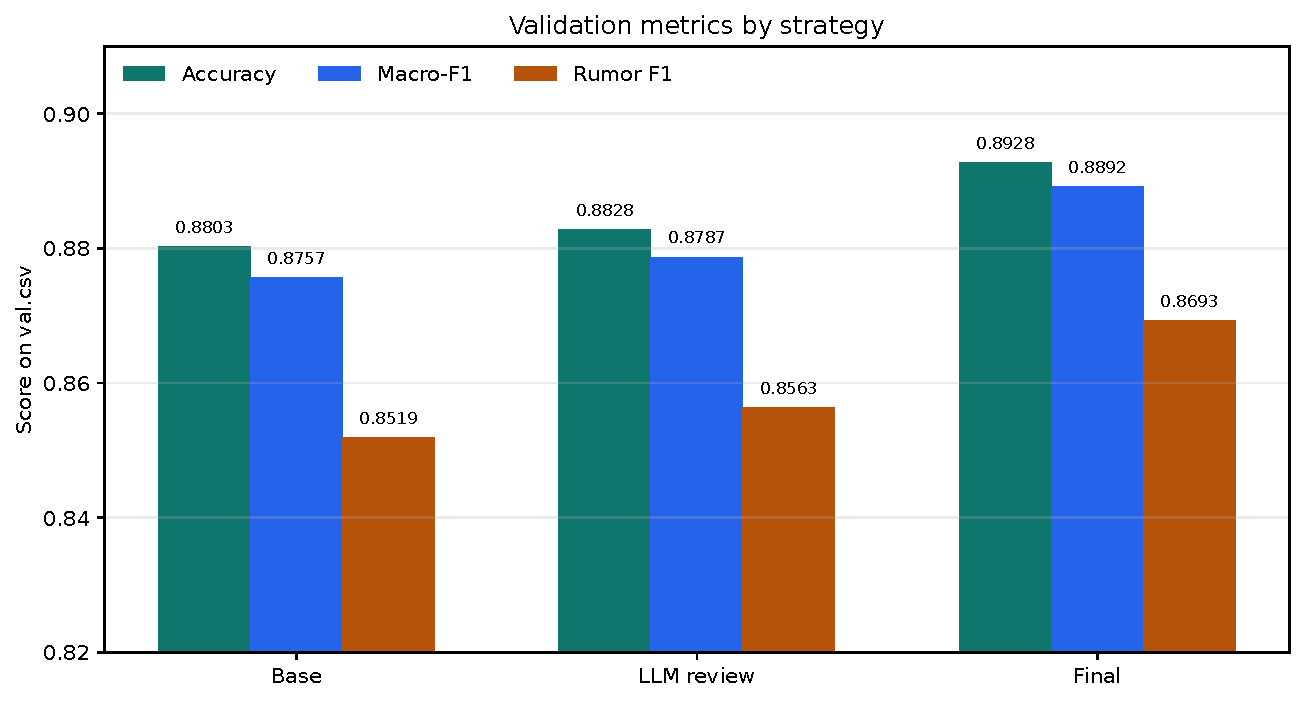
\includegraphics[width=\linewidth]{figures/metrics_overview.pdf}
\caption{主要指标对比}
\end{subfigure}
\hfill
\begin{subfigure}{0.49\textwidth}
\centering
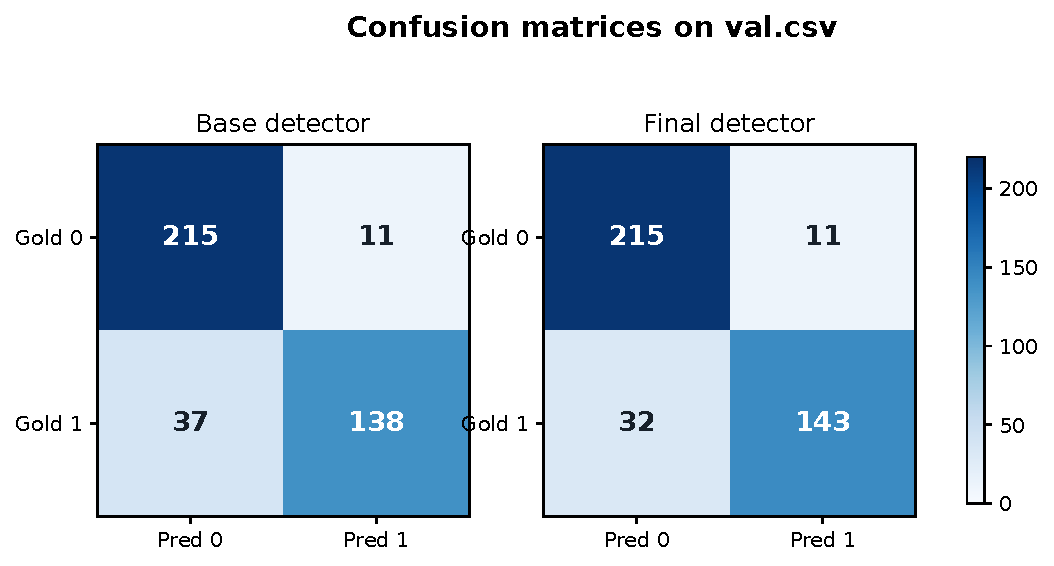
\includegraphics[width=\linewidth]{figures/confusion_matrices.pdf}
\caption{混淆矩阵对比}
\end{subfigure}
\caption{默认模型、LLM 复核与备选增强模型在验证集上的表现。}
\label{fig:metrics-cm}
\end{figure}

\begin{figure}[htbp]
\centering
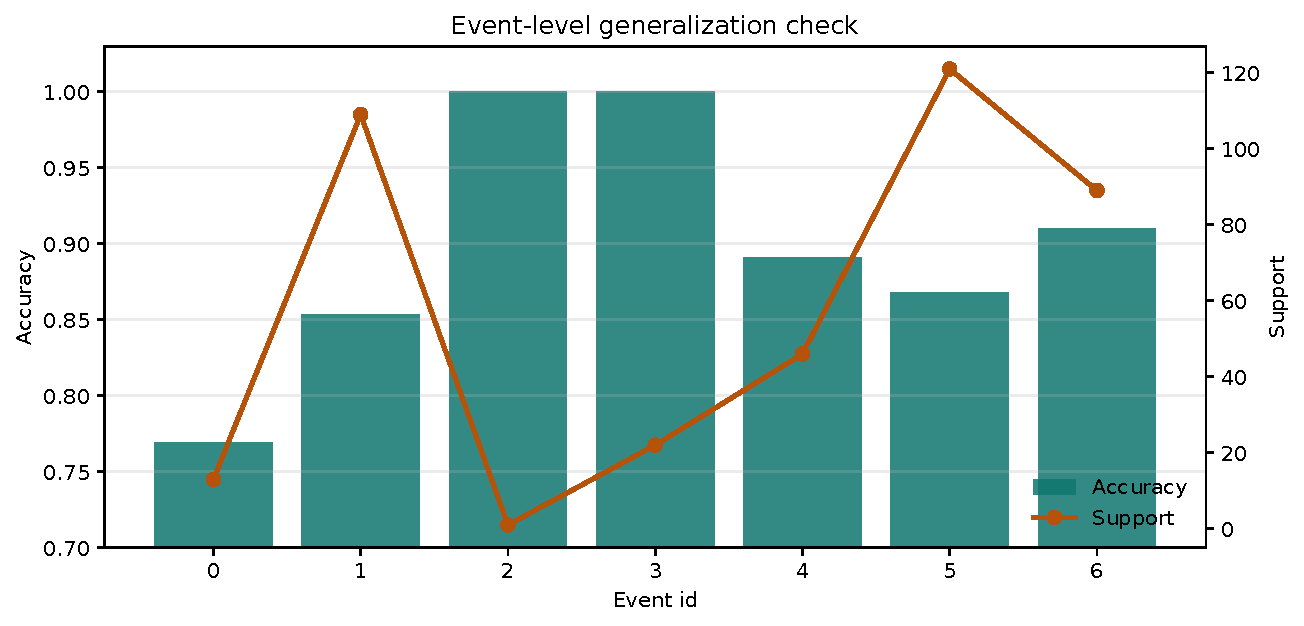
\includegraphics[width=0.70\textwidth]{figures/event_accuracy.pdf}
\caption{按 event 分组的准确率和样本量。event 0 与 event 1 的主要问题是 false negative，说明默认模型较保守，备选增强器主要针对这一错误模式。}
\label{fig:event-accuracy}
\end{figure}

判断依据固定包含预测标签、谣言概率、分类置信度、正向证据、反向证据和综合判断。由于证据来自 $w_i\phi_i(\tilde{x})$，解释与线性模型预测路径一致。前端页面把“输入文本-输出标签-输出解释”的链条可视化，方便检查模型来源和解释是否一致。对于规则增强样例，页面还同时展示基座模型原始预测和最终预测，避免把规则覆盖误理解为基座模型本身的直接输出。

\begin{figure}[htbp]
\centering
\begin{subfigure}{0.48\textwidth}
\centering
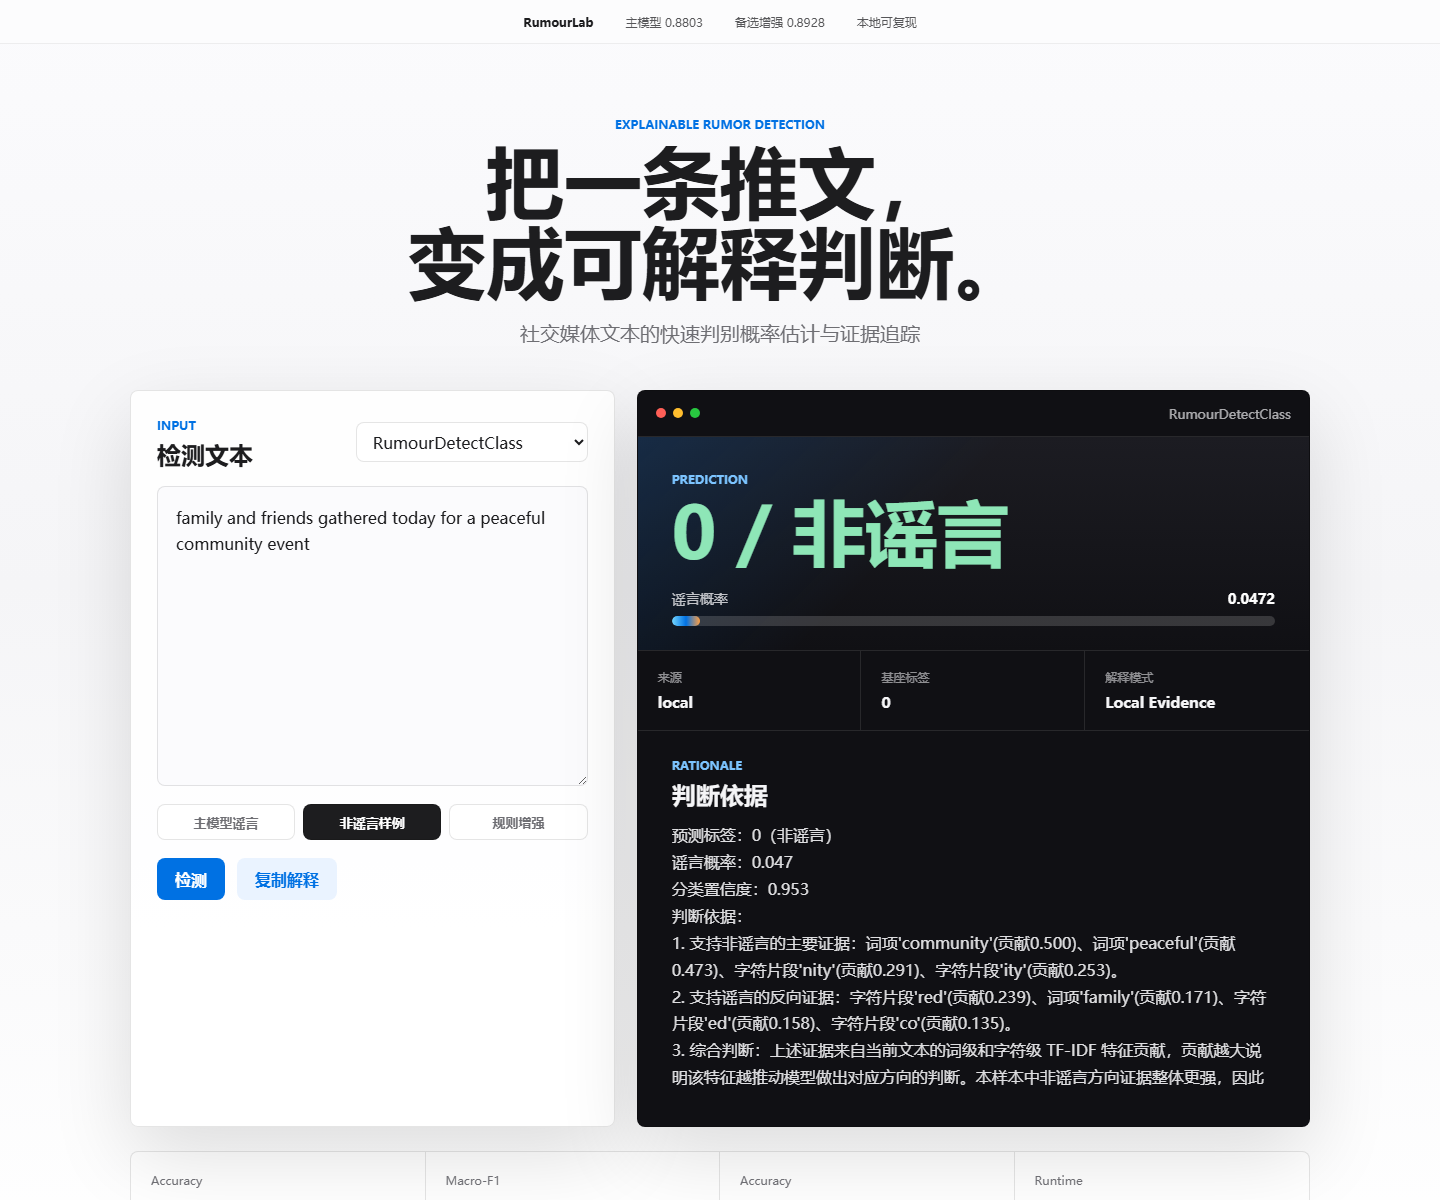
\includegraphics[width=\linewidth]{figures/demo_nonrumor_sample.png}
\caption{非谣言样例}
\end{subfigure}
\hfill
\begin{subfigure}{0.48\textwidth}
\centering
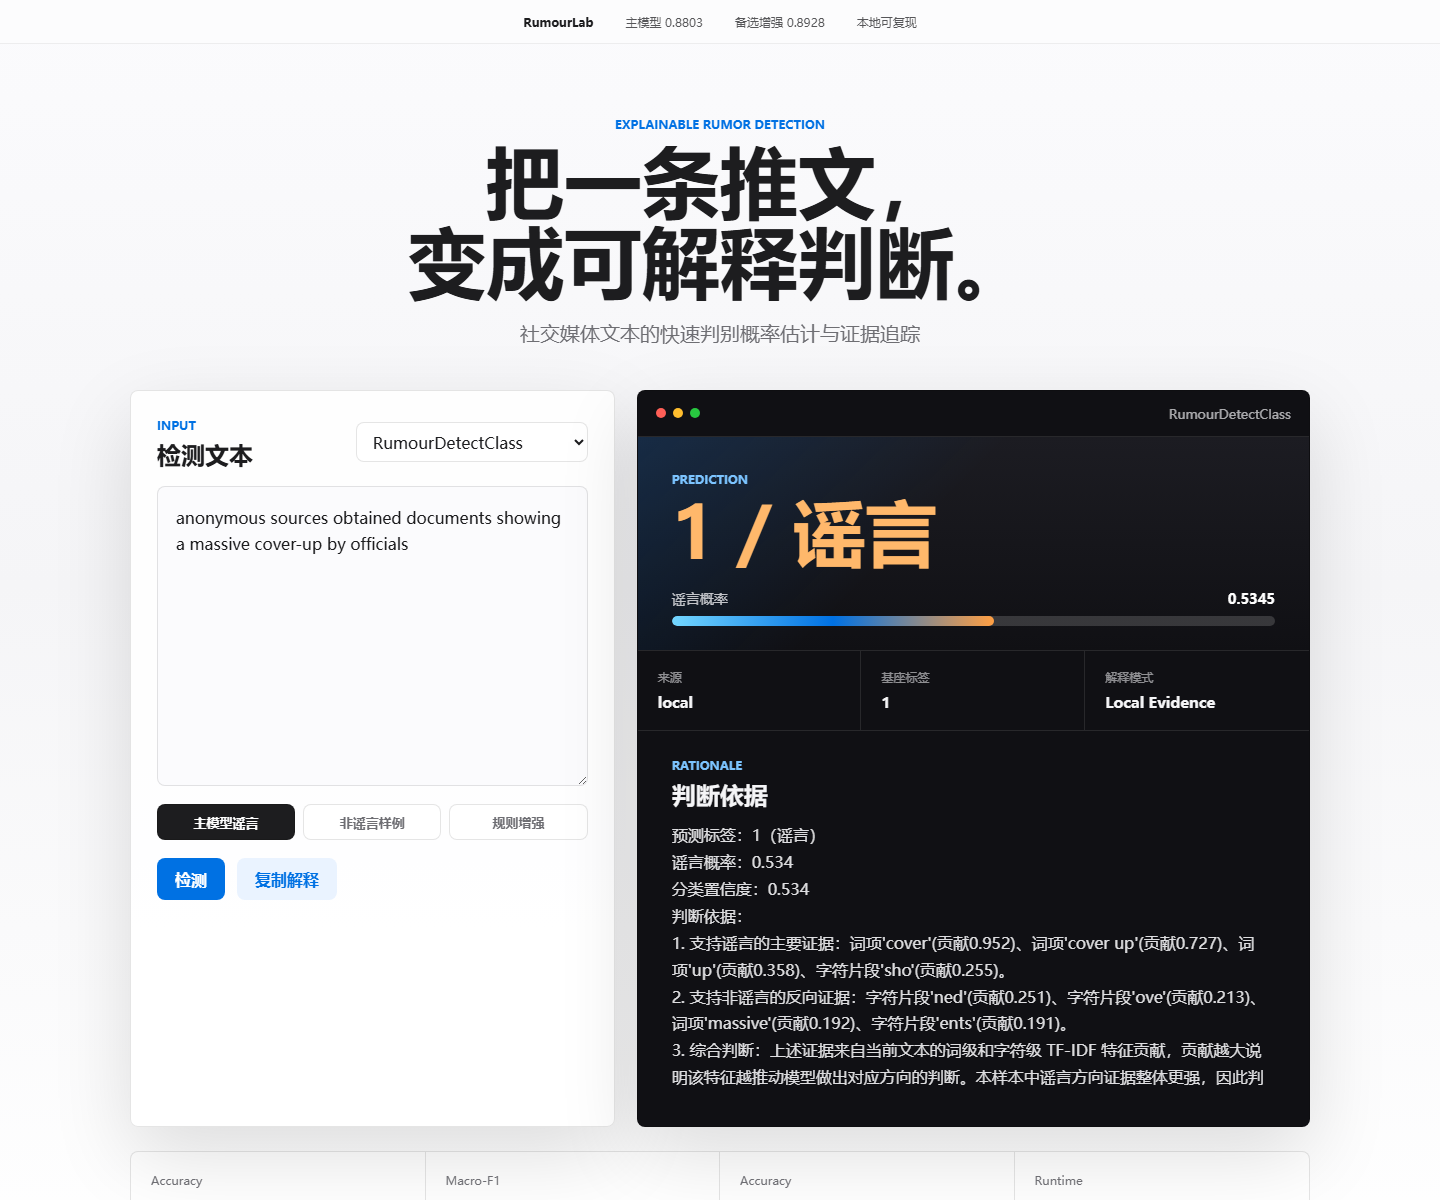
\includegraphics[width=\linewidth]{figures/demo_rumor_sample.png}
\caption{主模型谣言样例}
\end{subfigure}
\vspace{0.6em}
\begin{subfigure}{0.72\textwidth}
\centering
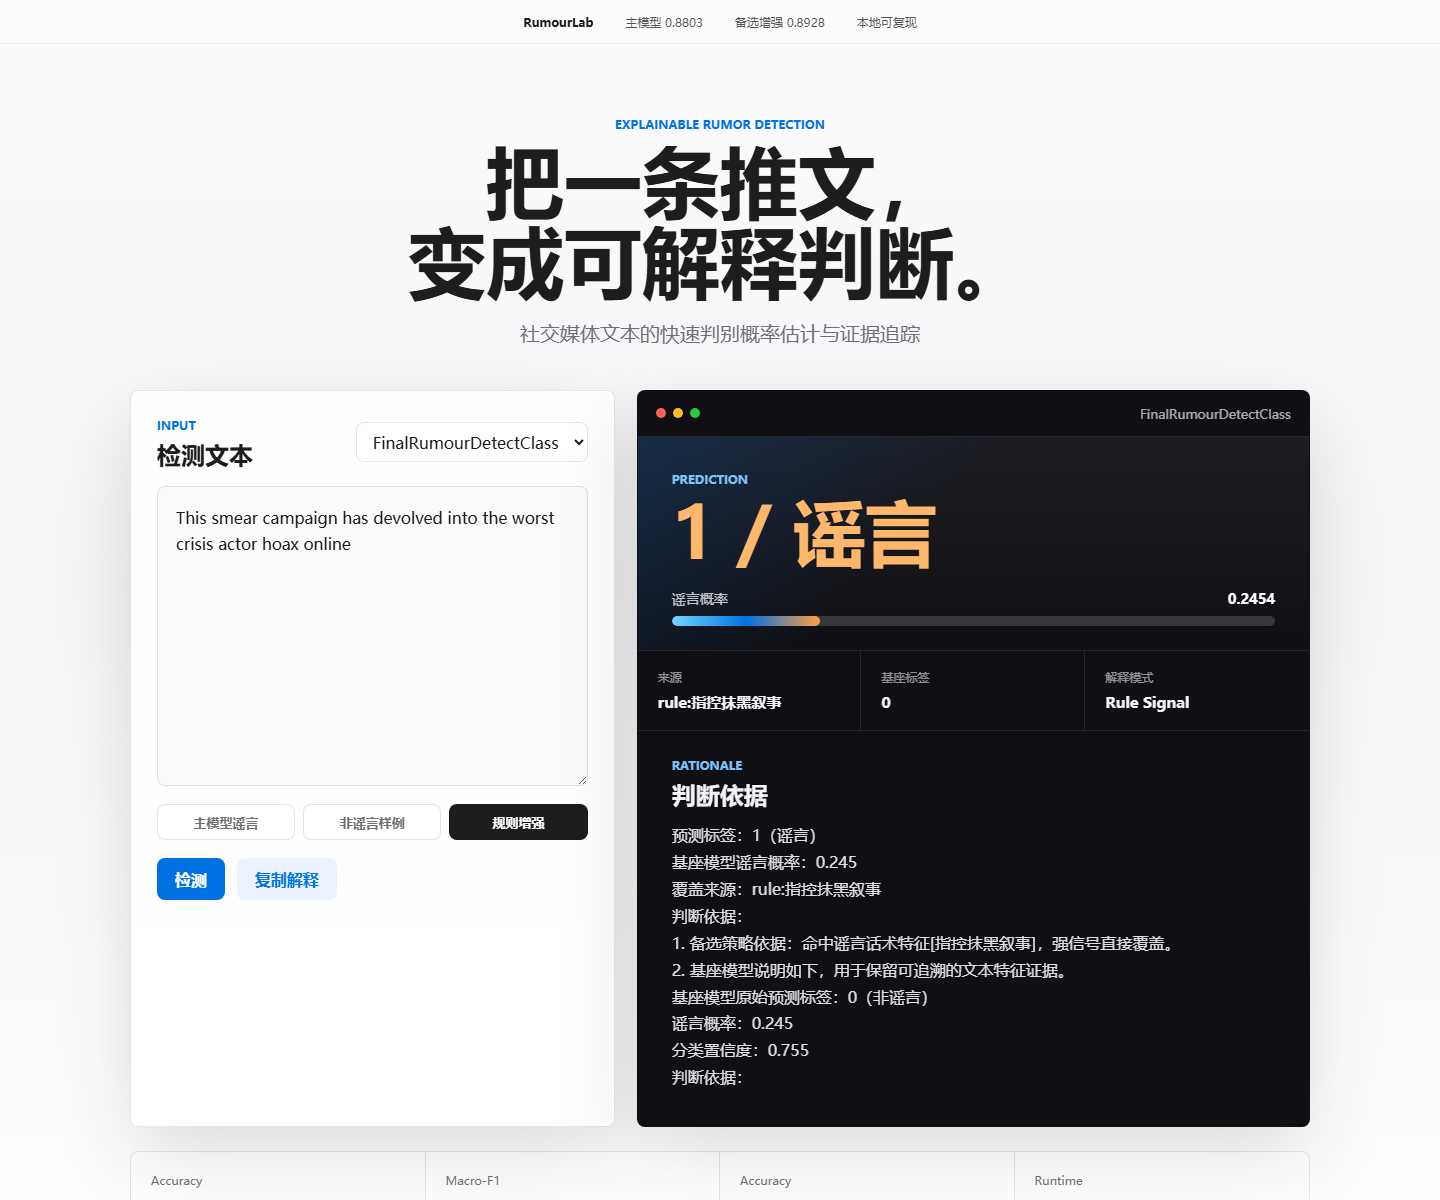
\includegraphics[width=\linewidth]{figures/demo_rule_enhanced.png}
\caption{规则增强样例}
\end{subfigure}
\caption{本地前端演示页面。新版页面将样例按钮拆分为“主模型谣言 / 非谣言样例 / 规则增强”，增加“复制解释”，并在增强模式中区分最终预测与基座模型原始预测。}
\label{fig:demo}
\end{figure}

\section{复现方式与提交检查}
教师复现默认主模型可执行：
\begin{lstlisting}[language=bash]
pip install -r requirements.txt
python -m src.train --with-explanations
python -m src.evaluate --show-examples 0
\end{lstlisting}
复现增强模型和前端可执行：
\begin{lstlisting}[language=bash]
python scripts/run_final_detector_evaluation.py
python scripts/run_demo_server.py
\end{lstlisting}

\begin{table}[H]
\centering
\caption{课程要求覆盖检查}
\begin{tabularx}{\textwidth}{L{3.6cm}Y}
\toprule
课程要求 & 覆盖情况 \\
\midrule
二分类输出 & \texttt{classify(text)} 输出 0/1，前端和预测文件同步展示。 \\
判断依据 & \texttt{explain(text)} 输出中文证据说明，图\ref{fig:demo}展示效果。 \\
检测结果分析图 & 已给出指标柱状图、混淆矩阵和事件级准确率图。 \\
代码可运行 & README、脚本和本节命令支持训练、评估、demo 与报告编译。 \\
小组分工 & 2.1 节写明分工，封面列出第 6 组成员和均等贡献。 \\
正文数量 & 正文约 2000 字。 \\
\bottomrule
\end{tabularx}
\end{table}

\section{工作总结}
\subsection{收获、心得}
本项目最大的收获是认识到“可解释”不只是生成自然语言，而是要让解释能追溯到模型证据。TF-IDF 线性模型虽然简单，但能清楚给出哪些词项或字符片段推动了预测；配合数据审计、错误分析和前端展示，可以形成完整、可复查的工程链路。我们也体会到，在课程作业中，稳定复现往往比堆叠复杂模型更重要：只要预处理、训练、评估和解释口径一致，轻量模型同样可以达到较好的效果，并且更容易清楚说明判断依据。

\subsection{遇到问题及解决思路}
主要问题有三类：第一，训练集中有同文本异标签冲突，我们通过一致预处理定位并只清洗训练集，同时保留原始数据，便于回溯；第二，默认模型 false negative 较多，我们尝试过阈值调整，但验证集效果下降，因此改为设计窄候选集增强器，避免过度规则覆盖；第三，LLM 直接接管标签不稳定，且依赖 API 与缓存，因此只作为可选复核和解释增强，不纳入默认依赖。第四，报告排版中长路径和大图容易造成溢出或空白，我们通过表格、子图和精简文字解决。

\section{课程建议}
建议后续课程提供隐藏测试集或统一评测脚本，减少对 \texttt{val.csv} 的过拟合空间；同时给出基础报告模板和结果文件命名规范，便于不同小组在准确率、解释性、运行时间和可复现性之间公平比较。若课程允许使用外部大模型，也建议明确其边界，例如是否可以参与最终标签判断、是否必须提供离线可复现模式、缓存文件能否作为评分依据。这样既能鼓励同学探索新方法，也能保证评分标准清晰。

\section{结论}
本项目实现了课程大作业所需的可解释谣言检测系统。默认主模型在 \texttt{val.csv} 上达到 Accuracy 0.8803，并输出基于局部特征贡献的中文解释；备选增强模型在不依赖 LLM 缓存的情况下达到 Accuracy 0.8928。报告中的数字均来自仓库结果文件或可复现实验脚本，并区分默认指标、增强实验和探索性记录。

\section*{参考文献}
\begin{enumerate}[label={[\arabic*]}]
\item 上海交通大学《人工智能导论》大作业说明与课程支持文档, 2026.
\item Shu K., Sliva A., Wang S., Tang J., Liu H. Fake News Detection on Social Media: A Data Mining Perspective. \textit{ACM SIGKDD Explorations}, 2017.
\item Salton G., Buckley C. Term-weighting approaches in automatic text retrieval. \textit{Information Processing \& Management}, 1988.
\item Pedregosa F. et al. Scikit-learn: Machine Learning in Python. \textit{Journal of Machine Learning Research}, 2011.
\end{enumerate}

\appendix
\section{核心接口示例}
\begin{lstlisting}[language=Python]
from src.rumor_detector import RumourDetectClass
from src.final_detector import FinalRumourDetectClass

main_detector = RumourDetectClass("models/rumor_ensemble.joblib")
label = main_detector.classify("input tweet text")
reason = main_detector.explain("input tweet text")

final_detector = FinalRumourDetectClass("models/rumor_ensemble.joblib")
result = final_detector.predict("input tweet text")
\end{lstlisting}

\end{document}

